\hypertarget{sistemas-supervisuxf3rios-scada-e-hmi}{%
\chapter{\texorpdfstring{Sistemas Supervisórios --- SCADA e HMI}{Sistemas Supervisórios  SCADA e HMI}}\label{sistemas-supervisuxf3rios-scada-e-hmi}}

\section*{Objetivos de Aprendizagem}

Ao final deste capítulo, o leitor será capaz de:

\begin{itemize}
\tightlist
\item
  Definir SCADA e distinguir suas funções principais.
\item
  Diferenciar SCADA, DCS e HMI local, reconhecendo quando usar cada um.
\item
  Identificar os principais softwares SCADA comerciais e open-source.
\item
  Descrever a evolução do SCADA: das primeiras gerações ao Cloud SCADA.
\end{itemize}

\begin{center}\rule{0.5\linewidth}{0.5pt}\end{center}

\hypertarget{o-que-uxe9-scada}{%
\section{O que é SCADA?}\label{o-que-uxe9-scada}}

\textbf{SCADA} (\emph{Supervisory Control and Data Acquisition} --- Controle Supervisório e Aquisição de Dados) é um sistema de software e hardware que permite \textbf{monitorar e controlar remotamente processos industriais e infraestruturas críticas} a partir de uma central de operações.

O nome descreve bem suas funções essenciais:

\begin{itemize}
\tightlist
\item
  \textbf{Supervisory Control:} permite que operadores visualizem o estado do processo e intervenham quando necessário --- ajustando setpoints, abrindo válvulas, desligando equipamentos.
\item
  \textbf{Data Acquisition:} coleta continuamente dados dos equipamentos de campo (CLPs, RTUs, transmissores) e os armazena em banco de dados histórico.
\end{itemize}

\begin{caixanota}

\textbf{Nota:} O SCADA \textbf{não realiza controle em malha fechada diretamente} na maioria das arquiteturas. Quem controla o processo em tempo real são os CLPs e DCSs no Nível 2. O SCADA supervisiona, centraliza e historiza --- e intervém de forma supervisória quando necessário.

\end{caixanota}

\begin{figure}
\centering
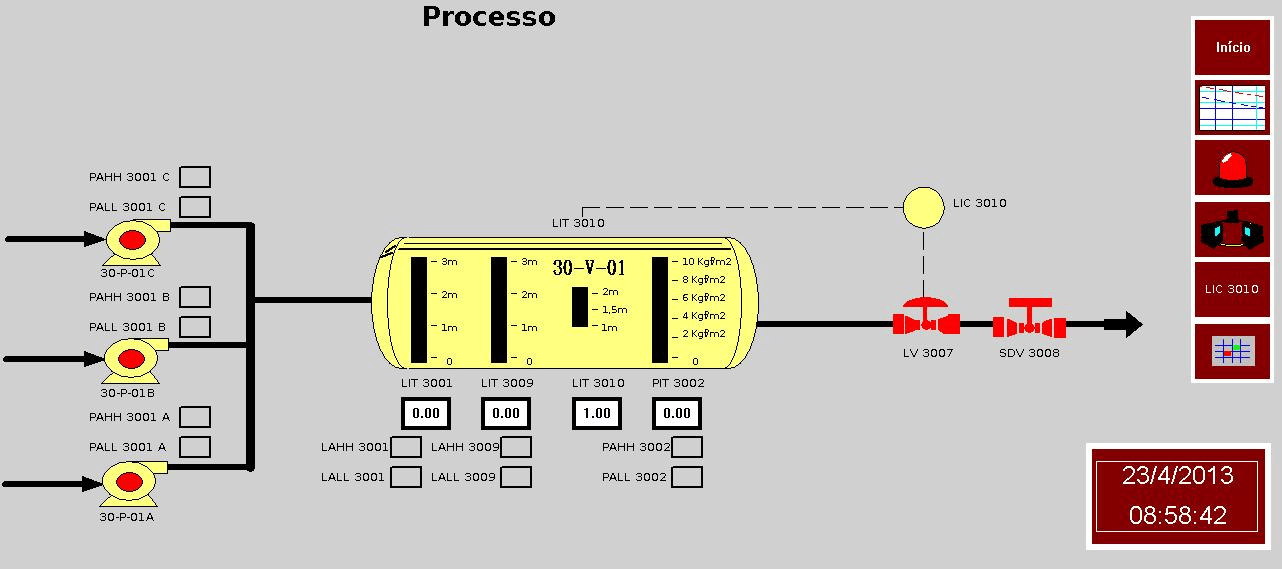
\includegraphics{../figuras/cap03-janela-ihm.png}
\caption[Figura 3.1 -- Janela de IHM de um sistema supervisório]{Figura 3.1 -- Janela de IHM de um sistema supervisório. \textbf{Fonte:} \emph{Livro SCADA --- versão para análise}, p.~51 (Machado, Pontes e Vianna, reproduzida com crédito).}
\end{figure}

A tela acima reúne os elementos que a ISA-101 --- principal referência global para o projeto de \textbf{IHM/SCADA de alta performance} (Seção 10.6.1) --- trata como camada de operação: o sinótico do
processo à esquerda, a \textbf{barra de navegação} à direita (acesso a processo, tendência, alarmes e
visão geral), a data e a hora de referência no canto inferior e a indicação de estado de cada
equipamento sobre o próprio desenho. Repare que a quantidade de informação é deliberadamente
pequena: o detalhamento pertence aos níveis de tela seguintes, não à visão de área --- princípio
desenvolvido no Capítulo 11.

\begin{center}\rule{0.5\linewidth}{0.5pt}\end{center}

\hypertarget{funuxe7uxf5es-principais-de-um-scada}{%
\section{Funções Principais de um SCADA}\label{funuxe7uxf5es-principais-de-um-scada}}

Um sistema SCADA moderno oferece as seguintes funções. Elas não são independentes: todas
dependem do mesmo conjunto de dados adquiridos do processo.

\begin{center}
\IfFileExists{../figuras/capitulo-03-m1.pdf}{%
  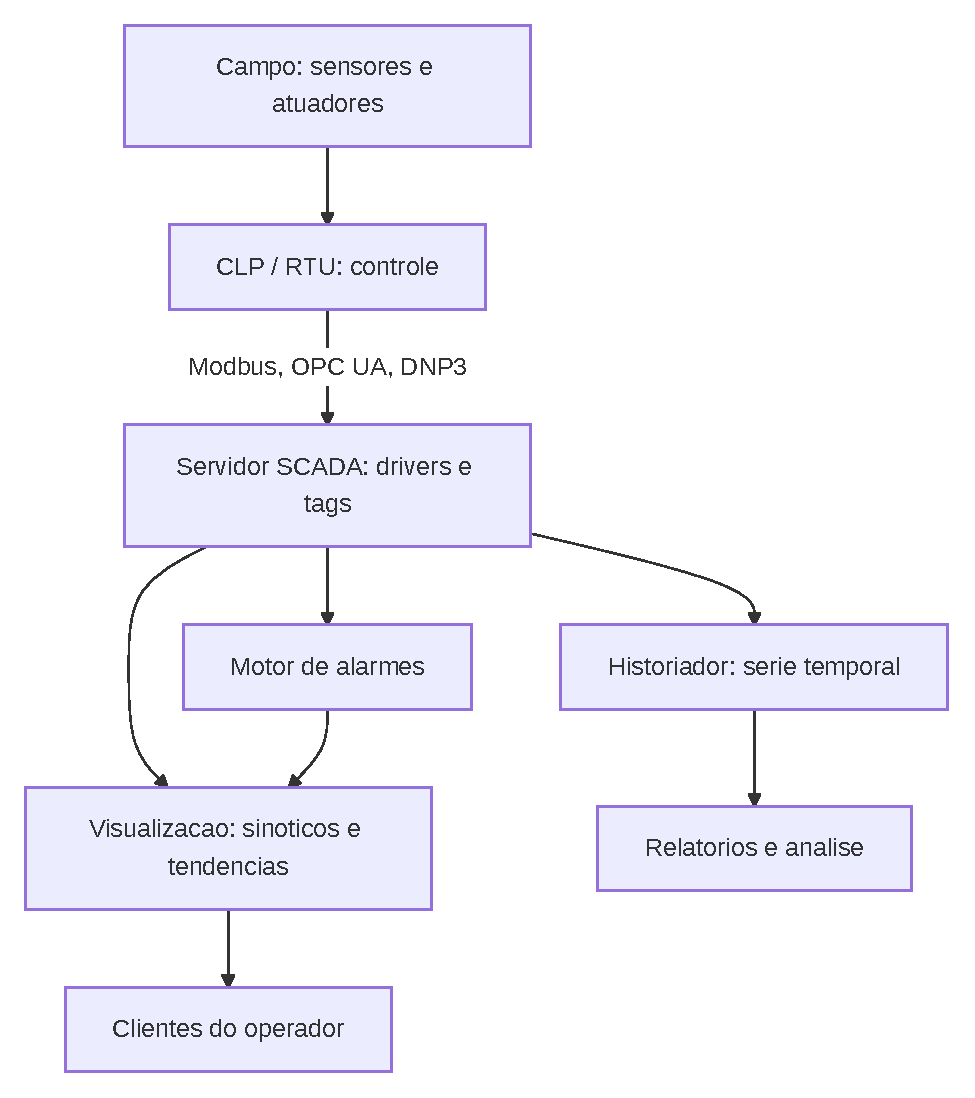
\includegraphics[width=\linewidth,height=0.8\textheight,keepaspectratio]{../figuras/capitulo-03-m1.pdf}%
}{\fbox{\parbox{0.9\linewidth}{\small Diagrama Mermaid ainda não renderizado: capitulo-03-m1. Rode scripts/render-mermaid.sh.}}}
\end{center}

\hypertarget{aquisiuxe7uxe3o-de-dados}{%
\subsection{Aquisição de Dados}\label{aquisiuxe7uxe3o-de-dados}}

Coleta cíclica de variáveis analógicas (temperatura, pressão, vazão) e digitais (status de bombas, posição de válvulas, alarmes) a partir dos equipamentos de campo. A frequência de coleta pode variar de milissegundos a minutos, dependendo da criticidade da variável.

\hypertarget{visualizauxe7uxe3o-hmi-centralizado}{%
\subsection{Visualização (HMI Centralizado)}\label{visualizauxe7uxe3o-hmi-centralizado}}

Apresentação gráfica do processo em \textbf{sinóticos} animados, onde:
- Válvulas mudam de cor conforme seu estado (aberta/fechada).
- Tanques e reatores mostram nível preenchido dinamicamente.
- Valores numéricos atualizam em tempo real.
- Gráficos de tendência mostram a evolução da variável ao longo do tempo.

\hypertarget{gerenciamento-de-alarmes}{%
\subsection{Gerenciamento de Alarmes}\label{gerenciamento-de-alarmes}}

\begin{itemize}
\tightlist
\item
  Detecção automática de condições anormais (variável fora de faixa, falha de equipamento, perda de comunicação).
\item
  Priorização de alarmes por criticidade (informativo, advertência, crítico, emergência).
\item
  Registro de alarmes com timestamp, operador responsável e ação tomada.
\item
  Relatórios de desempenho de alarmes (norma \textbf{EEMUA 191} e \textbf{ISA-18.2}).
\end{itemize}

\begin{caixaatencao}

\textbf{Atenção:} Sistemas SCADA mal configurados podem gerar \textbf{inundação de alarmes} (\emph{alarm flooding}) --- situações em que centenas de alarmes disparam simultaneamente, dificultando a identificação da causa raiz. O gerenciamento racional de alarmes é uma disciplina de engenharia por si só.

\end{caixaatencao}

\hypertarget{controle-supervisuxf3rio}{%
\subsection{Controle Supervisório}\label{controle-supervisuxf3rio}}

O operador pode enviar comandos ao processo através do SCADA:
- Alteração de setpoints de controladores PID.
- Abertura/fechamento de válvulas on/off.
- Partida e parada de motores.
- Execução de sequências de operação.

\hypertarget{historizauxe7uxe3o}{%
\subsection{Historização}\label{historizauxe7uxe3o}}

Armazenamento de séries temporais de dados de processo em banco de dados otimizado para esse fim. Permite:
- Análise de tendências históricas.
- Investigação de incidentes (reconstrução do evento).
- Relatórios de produção.
- Alimentação de sistemas de analytics e IA.

\textbf{Bancos de dados de processo populares:} OSIsoft PI System (agora AVEVA PI), Honeywell Uniformance, InfluxDB (open-source), TimescaleDB.

\hypertarget{relatuxf3rios}{%
\subsection{Relatórios}\label{relatuxf3rios}}

Geração automática de relatórios operacionais, de qualidade e de desempenho de equipamentos (OEE), em formatos PDF, Excel ou dashboards web.

\begin{caixafigura}

\textbf{{[}Figura 3.2 -- Funções de um SCADA moderno{]}}
\emph{Diagrama circular ou de hexágonos com as seis funções: Aquisição de Dados, Visualização, Alarmes, Controle, Historização e Relatórios --- com ícones representativos para cada uma. No centro, o logo ou nome do sistema SCADA.}

\end{caixafigura}

\begin{center}\rule{0.5\linewidth}{0.5pt}\end{center}

\hypertarget{scada-dcs-hmi-local}{%
\section{\texorpdfstring{SCADA \ensuremath{\times} DCS \ensuremath{\times} HMI Local}{SCADA  DCS  HMI Local}}\label{scada-dcs-hmi-local}}

Uma dúvida comum entre estudantes e profissionais é a diferença entre SCADA, DCS e HMI. A \textbf{Tabela 3.1} resume as principais distinções:

\textbf{Tabela 3.1 -- Comparativo SCADA \ensuremath{\times} DCS \ensuremath{\times} HMI Local}

\begin{longtable}[]{@{}
  >{\raggedright\arraybackslash}p{(\columnwidth - 6\tabcolsep) * \real{0.2500}}
  >{\raggedright\arraybackslash}p{(\columnwidth - 6\tabcolsep) * \real{0.2500}}
  >{\raggedright\arraybackslash}p{(\columnwidth - 6\tabcolsep) * \real{0.2500}}
  >{\raggedright\arraybackslash}p{(\columnwidth - 6\tabcolsep) * \real{0.2500}}@{}}
\toprule\noalign{}
\begin{minipage}[b]{\linewidth}\raggedright
Critério
\end{minipage} & \begin{minipage}[b]{\linewidth}\raggedright
HMI Local
\end{minipage} & \begin{minipage}[b]{\linewidth}\raggedright
SCADA
\end{minipage} & \begin{minipage}[b]{\linewidth}\raggedright
DCS
\end{minipage} \\
\midrule\noalign{}
\endhead
\bottomrule\noalign{}
\endlastfoot
\textbf{Escopo} & Um equipamento ou célula & Planta inteira ou múltiplos sites & Processo contínuo integrado \\
\textbf{Localização} & Junto ao equipamento & Sala de controle centralizada & Sala de controle + campo \\
\textbf{Controle} & Visualização + comandos locais & Supervisório (via CLP/RTU) & Controle distribuído nativo \\
\textbf{Conectividade} & Serial, Ethernet & WAN, rádio, fibra, 4G & Rede proprietária de campo \\
\textbf{Histórico} & Limitado ou nenhum & Banco de dados de processo & Banco de dados integrado \\
\textbf{Redundância} & Geralmente sem & Servidores redundantes & Redundância total nativa \\
\textbf{Aplicação típica} & Máquina CNC, bomba, compressor & Oleoduto, ETAP, subestação & Refinaria, petroquímica, papel e celulose \\
\textbf{Custo relativo} & Baixo & Médio & Alto \\
\end{longtable}

\begin{caixadica}

\textbf{Dica:} Na prática moderna, as fronteiras entre SCADA e DCS estão se apagando. Sistemas como AVEVA System Platform e Honeywell Experion são, simultaneamente, SCADA e DCS --- com controle nativo distribuído e supervisão centralizada na mesma plataforma.

\end{caixadica}

\begin{center}\rule{0.5\linewidth}{0.5pt}\end{center}

\hypertarget{gerauxe7uxf5es-do-scada}{%
\section{Gerações do SCADA}\label{gerauxe7uxf5es-do-scada}}

A evolução do SCADA ocorreu em quatro gerações bem definidas:

\textbf{Geração 1 --- Monolítico (anos 1970--1980)}
- Sistemas proprietários, sem conectividade entre sistemas.
- Hardware dedicado de cada fabricante (protocolos fechados).
- Computadores de grande porte (\emph{mainframes}) ou minicomputadores.

\textbf{Geração 2 --- Distribuído (anos 1980--1990)}
- Redes locais (LANs) conectam múltiplas estações de trabalho.
- Aparecimento dos primeiros padrões abertos (Modbus, RS-485).
- Servidores Unix e estações Sun Sparc.

\textbf{Geração 3 --- Em Rede (anos 1990--2000)}
- Adoção da infraestrutura Ethernet e TCP/IP.
- OPC (OLE for Process Control) como padrão de integração.
- Interfaces gráficas Windows, banco de dados SQL.

\textbf{Geração 4 --- IoT / Cloud SCADA (2010--presente)}
- Integração nativa com IIoT, MQTT, OPC UA.
- SCADA como serviço (SaaS) na nuvem.
- Acesso via navegador web e aplicativos móveis.
- Analytics, Machine Learning e IA embarcados.

\begin{figure}
\centering
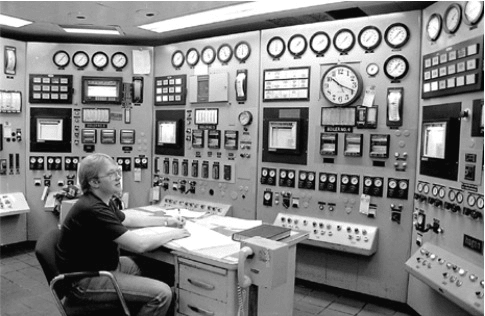
\includegraphics{../figuras/cap03-sala-convencional.png}
\caption[Figura 3.3 -- Sala de controle com painel de instrumentos convencionais]{Figura 3.3 -- Sala de controle com painel de instrumentos convencionais. \textbf{Fonte:} \emph{Livro SCADA --- versão para análise}, p.~15 (fotografia de Solomon, 2005, adaptada pelos autores).}
\end{figure}

A cena corresponde à geração \textbf{anterior} ao SCADA: cada variável tem um mostrador dedicado
no painel e o histórico do processo existe apenas na pena do registrador. Substituir esse painel
por estações de supervisão reduziu o espaço físico da sala de controle e transferiu a informação
para um banco de dados único --- a mudança que a Seção 3.4 descreve em quatro gerações.

Cada geração resolveu o problema da anterior e criou o seu próprio:

\begin{center}
\IfFileExists{../figuras/capitulo-03-m2.pdf}{%
  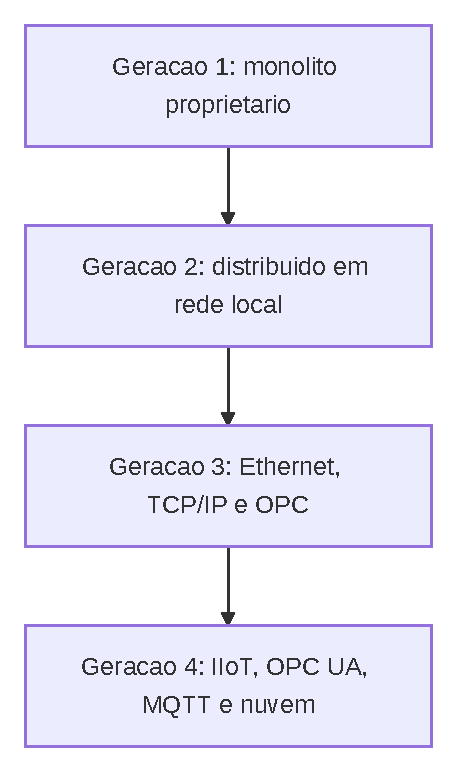
\includegraphics[width=\linewidth,height=0.8\textheight,keepaspectratio]{../figuras/capitulo-03-m2.pdf}%
}{\fbox{\parbox{0.9\linewidth}{\small Diagrama Mermaid ainda não renderizado: capitulo-03-m2. Rode scripts/render-mermaid.sh.}}}
\end{center}

\begin{center}\rule{0.5\linewidth}{0.5pt}\end{center}

\hypertarget{principais-plataformas-scada}{%
\section{Principais Plataformas SCADA}\label{principais-plataformas-scada}}

\hypertarget{plataformas-comerciais}{%
\subsection{Plataformas Comerciais}\label{plataformas-comerciais}}

\textbf{AVEVA System Platform (ex-Wonderware)}
- Uma das plataformas mais difundidas globalmente.
- Arquitetura de objetos reutilizáveis (Application Server).
- Forte integração com o AVEVA PI System para historização.

\textbf{Ignition (Inductive Automation)}
- Licenciamento por servidor (não por tag), modelo altamente econômico.
- Baseado em Java, com designer web --- sem instalação no cliente.
- Módulos para SCADA, IIoT (MQTT), MES e relatórios.
- Comunidade open-source ativa.

\textbf{Rockwell FactoryTalk View}
- Nativo do ecossistema Allen-Bradley/Rockwell Automation.
- Excelente integração com CLPs ControlLogix e CompactLogix.

\textbf{Siemens WinCC}
- Integrado ao TIA Portal.
- Versões para HMI local (WinCC flexible) e SCADA (WinCC SCADA / WinCC OA).

\textbf{Honeywell Experion PKS}
- Plataforma DCS+SCADA integrada para grandes processos contínuos.

\hypertarget{plataformas-open-source-e-gratuitas}{%
\subsection{Plataformas Open-Source e Gratuitas}\label{plataformas-open-source-e-gratuitas}}

\begin{longtable}[]{@{}
  >{\raggedright\arraybackslash}p{(\columnwidth - 4\tabcolsep) * \real{0.3333}}
  >{\raggedright\arraybackslash}p{(\columnwidth - 4\tabcolsep) * \real{0.3333}}
  >{\raggedright\arraybackslash}p{(\columnwidth - 4\tabcolsep) * \real{0.3333}}@{}}
\toprule\noalign{}
\begin{minipage}[b]{\linewidth}\raggedright
Plataforma
\end{minipage} & \begin{minipage}[b]{\linewidth}\raggedright
Características
\end{minipage} & \begin{minipage}[b]{\linewidth}\raggedright
Ideal para
\end{minipage} \\
\midrule\noalign{}
\endhead
\bottomrule\noalign{}
\endlastfoot
\textbf{ScadaBR} & Brasileira, baseada em Java, suporte a Modbus/DNP3/SNMP & Projetos educacionais e PMEs \\
\textbf{OpenSCADA} & Linux-first, modular, suporte a SNMP e Modbus & Ambientes Linux industriais \\
\textbf{Node-RED} & Programação visual (flow-based), extensível, leve & IIoT, prototipagem, supervisão simples \\
\textbf{Grafana + InfluxDB} & Dashboard + banco de dados de série temporal & Visualização e analytics de dados históricos \\
\end{longtable}

\begin{caixanota}

\textbf{Nota:} O \textbf{ScadaBR} é especialmente relevante no contexto educacional brasileiro por ser open-source, em português e já ter sido utilizado em projetos de pesquisa em diversas universidades brasileiras. O Node-RED é detalhado no Capítulo 7.

\end{caixanota}

\begin{center}\rule{0.5\linewidth}{0.5pt}\end{center}

\hypertarget{requisitos-para-implantauxe7uxe3o-de-um-scada}{%
\section{Requisitos para Implantação de um SCADA}\label{requisitos-para-implantauxe7uxe3o-de-um-scada}}

Ao especificar e implantar um sistema SCADA, os seguintes aspectos devem ser considerados:

\textbf{Tabela 3.2 -- Checklist de especificação de um SCADA}

\begin{longtable}[]{@{}ll@{}}
\toprule\noalign{}
Aspecto & Questões a Responder \\
\midrule\noalign{}
\endhead
\bottomrule\noalign{}
\endlastfoot
\textbf{Escopo} & Quantos pontos (tags)? Quantos sites? \\
\textbf{Conectividade} & Quais protocolos os CLPs/RTUs usam? \\
\textbf{Disponibilidade} & É necessária redundância de servidores? \\
\textbf{Usuários} & Quantos clientes simultâneos? Acesso remoto? \\
\textbf{Histórico} & Quais variáveis historizar? Por quanto tempo? \\
\textbf{Alarmes} & Quantos alarmes? Notificação por email/SMS? \\
\textbf{Relatórios} & Quais relatórios são obrigatórios (regulatórios)? \\
\textbf{Segurança} & Controle de acesso por perfil de usuário? \\
\textbf{Integração} & Interface com MES/ERP? \\
\textbf{Normas} & IEC 62264, ISA-18.2, LGPD (dados de operadores)? \\
\end{longtable}

\begin{center}\rule{0.5\linewidth}{0.5pt}\end{center}

\hypertarget{estudo-de-caso-migrauxe7uxe3o-de-um-scada-de-gerauxe7uxe3o-3-para-gerauxe7uxe3o-4}{%
\section{\texorpdfstring{Estudo de Caso --- Migração de um SCADA de geração 3 para geração 4}{Estudo de Caso  Migração de um SCADA de geração 3 para geração 4}}\label{estudo-de-caso-migrauxe7uxe3o-de-um-scada-de-gerauxe7uxe3o-3-para-gerauxe7uxe3o-4}}

\textbf{Cenário.} Distribuidora de água com 42 estações de bombeamento, elevatórias e reservatórios
distribuídos em quatro municípios. O SCADA atual é de geração 3: rodou sobre Windows Server
2003, com OPC DA e drivers proprietários de dois fabricantes de RTU. O sistema funciona --- o
problema é que ninguém consegue mantê-lo.

\textbf{Sintomas que dispararam o projeto.}

\begin{itemize}
\tightlist
\item
  \textbf{Máquina virtual parada de atualizar} três anos, sem fornecedor para o sistema operacional.
\item
  \textbf{Um engenheiro} na equipe domina o pacote antigo; as demais pessoas dependem dele.
\item
  \textbf{Dados presos}: o historiador é proprietário e não aceita consulta externa, o que impede
  qualquer análise no Grafana ou no Excel.
\item
  \textbf{Integração impossível}: o novo sistema corporativo de manutenção não fala OPC DA, e não há
  caminho para levar dados das RTUs até ele.
\end{itemize}

\textbf{Estratégia adotada --- em camadas, não em big bang.}

\begin{longtable}[]{@{}
  >{\raggedright\arraybackslash}p{(\columnwidth - 4\tabcolsep) * \real{0.3333}}
  >{\raggedright\arraybackslash}p{(\columnwidth - 4\tabcolsep) * \real{0.3333}}
  >{\raggedright\arraybackslash}p{(\columnwidth - 4\tabcolsep) * \real{0.3333}}@{}}
\toprule\noalign{}
\begin{minipage}[b]{\linewidth}\raggedright
Etapa
\end{minipage} & \begin{minipage}[b]{\linewidth}\raggedright
Movimento
\end{minipage} & \begin{minipage}[b]{\linewidth}\raggedright
Efeito imediato
\end{minipage} \\
\midrule\noalign{}
\endhead
\bottomrule\noalign{}
\endlastfoot
1 & \emph{Gateway} OPC UA na frente dos drivers antigos & Moderniza a interface sem tocar nas RTUs \\
2 & Novo servidor SCADA em paralelo, com OPC UA & Operação continua no sistema antigo \\
3 & Espelhamento do histórico para banco de séries temporais & Dados deixam de ficar presos \\
4 & Migração de telas em blocos, por área & Cada área migra e é validada separadamente \\
5 & Desligamento do sistema antigo, mantido em leitura por 6 meses & Saída reversível \\
\end{longtable}

\textbf{O que observar no resultado.} A etapa 1 é a que destrava o projeto: um \emph{gateway} de protocolo
converte o que existe \textbf{sem exigir substituição de campo}. É o padrão descrito na Seção 5.4 e
reaproveitado no Capítulo 13 --- raramente a migração começa pelo equipamento mais caro.

\textbf{Limitações do arranjo.} O \emph{gateway} é mais um ponto de falha e precisa de supervisão própria:
se ele para, o dado para, mesmo com CLP e rede em pleno funcionamento. Além disso, migrar telas em
blocos só funciona se as duas gerações coexistirem por um período --- o que exige disciplina de
numeração de tags e de \emph{timestamps} entre os dois ambientes.

\begin{center}\rule{0.5\linewidth}{0.5pt}\end{center}

\hypertarget{resumo}{%
\section{Resumo}\label{resumo}}

\begin{itemize}
\tightlist
\item
  \textbf{SCADA} é um sistema de supervisão centralizada que combina aquisição de dados, visualização gráfica, gerenciamento de alarmes, controle supervisório e historização.
\item
  \textbf{SCADA} difere do \textbf{DCS} (que controla diretamente o processo) e da \textbf{HMI local} (escopo restrito a um equipamento).
\item
  O SCADA evoluiu em quatro gerações: de sistemas monolíticos proprietários (anos 70) a plataformas cloud-native com IIoT (hoje).
\item
  Plataformas líderes incluem AVEVA, Ignition e Siemens WinCC; no segmento open-source, destacam-se ScadaBR e Node-RED.
\end{itemize}

\begin{center}\rule{0.5\linewidth}{0.5pt}\end{center}

\hypertarget{questuxf5es-de-revisuxe3o}{%
\section{Questões de Revisão}\label{questuxf5es-de-revisuxe3o}}

\textbf{Conceituais:}

\begin{enumerate}
\def\labelenumi{\arabic{enumi}.}
\tightlist
\item
  Expanda a sigla SCADA e explique o significado de cada palavra.
\item
  Quais são as seis funções principais de um sistema SCADA moderno? Descreva duas delas.
\item
  Qual é a diferença entre um sistema DCS e um SCADA? Em qual situação você escolheria um DCS em vez de um SCADA?
\end{enumerate}

\textbf{Práticas:}

\begin{enumerate}
\def\labelenumi{\arabic{enumi}.}
\setcounter{enumi}{3}
\tightlist
\item
  Uma distribuidora de água deseja implantar um sistema para monitorar remotamente 50 estações de bombeamento distribuídas em um município, com histórico de consumo, alarmes de falhas e acesso web para a equipe de manutenção. Qual tipo de sistema (HMI local, SCADA ou DCS) e qual plataforma você recomendaria? Justifique.
\item
  O que é ``alarm flooding'' e quais práticas de engenharia podem ser adotadas para evitá-lo?
\end{enumerate}

\textbf{Desafio:}

\begin{enumerate}
\def\labelenumi{\arabic{enumi}.}
\setcounter{enumi}{5}
\tightlist
\item
  Compare o modelo de licenciamento do SCADA Ignition (por servidor, tags ilimitados) com o modelo tradicional por número de tags (ex.: AVEVA). Quais são as vantagens e desvantagens de cada modelo para uma empresa que está expandindo sua operação?
\end{enumerate}

\begin{center}\rule{0.5\linewidth}{0.5pt}\end{center}

\hypertarget{referuxeancias}{%
\section{Referências}\label{referuxeancias}}

\begin{itemize}
\tightlist
\item
  BOYER, S. A. \emph{SCADA: Supervisory Control and Data Acquisition}. 4. ed.~ISA, 2010.
\item
  ISA-18.2: \emph{Management of Alarm Systems for the Process Industries}. ISA, 2016.
\item
  EEMUA Publication 191: \emph{Alarm Systems --- A Guide to Design, Management and Procurement}. EEMUA, 2013.
\item
  INDUCTIVE AUTOMATION. \emph{Ignition SCADA Platform}. Disponível em: inductiveautomation.com.
\item
  AVEVA. \emph{System Platform Overview}. Disponível em: aveva.com.
\item
  MACHADO, C. F. B.; PONTES, M. O.; VIANNA, W. S. \emph{SCADA --- Supervisory Control and Data
  Acquisition: sistemas de supervisão e aquisição de dados para automação}. (Material de origem desta
  apostila; figuras dos autores reproduzidas com crédito.)
\end{itemize}
